\subsection{Progettazione architetturale}

\subsubsection{Prospetto orario}
Nel periodo di progettazione architetturale la distribuzione oraria è la seguente:

\renewcommand{\arraystretch}{1.5}
\begin{table}[H]
\begin{center}
\begin{tabular}{|c|c|c|c|c|c|c|c|}
\hline
\rowcolor{title_row}
\textbf{\color{title_text}{Nome}} & \textbf{\color{title_text}{Resp.}} & \textbf{\color{title_text}{Ammi.}} & \textbf{\color{title_text}{Analist.}} & \textbf{\color{title_text}{Progett.}} & \textbf{\color{title_text}{Program.}} & \textbf{\color{title_text}{Verific.}} & \textbf{\color{title_text}{Totale}} \\ \hline
Andrea Trevisin  & & & & 14 & 6 & 12 & 32 \\ \hline
Giacomo Barzon   &  & 4 &  & 10 & 8 & 8 & 30\\ \hline
Giovanni Sorice  & 8 &  &  & 10 & 6 & 8 & 32\\ \hline
Lorenzo Busin    &  & 3  &  & 12 & 8 & 10 & 33\\ \hline
Marco Costantino & 6 &  &  &  & 10 & 14 & 30\\ \hline
Michele Roverato &  & 6 & 8 &  & 8 & 10 & 32\\ \hline
Nicolò Tartaggia &  & 5  & 8 &  & 10 & 8 & 31\\ \hline
\end{tabular}
\caption{Tabella 5.3.1: Distribuzione oraria del periodo "Progettazione architetturale"\label{}}
\end{center}
\end{table}
\renewcommand{\arraystretch}{1}

Il seguente grafico dà una rappresentazione visiva della suddivisione oraria: \\
\begin{figure} [H]
	\centering
	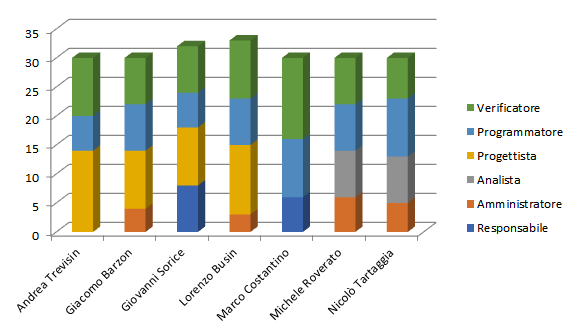
\includegraphics[scale=1]{Res/ExcelGrafici/Grafici/ProgettazioneOre.png}
	\caption{Figura 5.3.1: Grafico suddivisione oraria del periodo "Progettazione architetturale"}\label{}
\end{figure}


\subsubsection{Prospetto economico}
Nel periodo di progettazione architetturale il resoconto della distribuzione delle ore e dei relativi costi è la seguente:

\renewcommand{\arraystretch}{1.5}
\begin{table}[H]
\begin{center}
\begin{tabular}{|c|c|c|}
\hline
\rowcolor{title_row}
\textbf{\color{title_text}{Ruolo}}  & \textbf{\color{title_text}{Ore}} & \textbf{\color{title_text}{Costo in \euro}} \\ \hline
Responsabile    & 14              & 420                     \\ \hline
Amministratore  & 18              & 360                   \\ \hline
Analista        & 16              & 400                    \\ \hline
Progettista     & 46              & 1.012                     \\ \hline
Programmatore   & 56              & 840                     \\ \hline
Verificatore    & 70              & 1.050                    \\ \hline
\textbf{Totale} & \textbf{220}    & \textbf{4.082}         \\ \hline
\end{tabular}
\caption{Tabella 5.3.2: Prospetto economico del periodo "Progettazione architetturale"\label{}}
\end{center}
\end{table}
\renewcommand{\arraystretch}{1}

Il seguente grafico dà una rappresentazione visiva della distribuzione dei ruoli: \\
\begin{figure} [H]
	\centering
	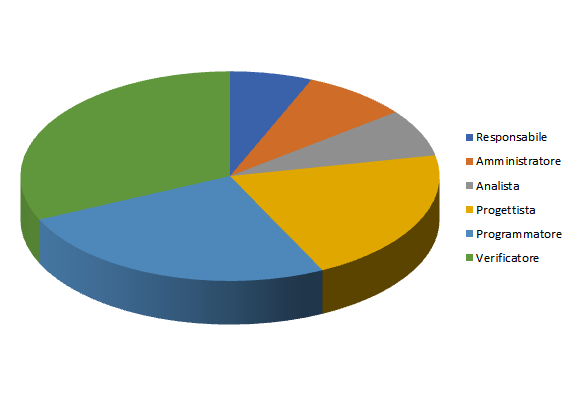
\includegraphics[scale=1]{Res/ExcelGrafici/Grafici/ProgettazioneRuoli.png}
	\caption{Figura 5.3.2: Grafico suddivisione dei ruoli del periodo "Progettazione architetturale"}\label{}
\end{figure}

\pagebreak
